
\usetikzlibrary{arrows.meta,shapes.misc}
\begin{frame}{sending two at a time}
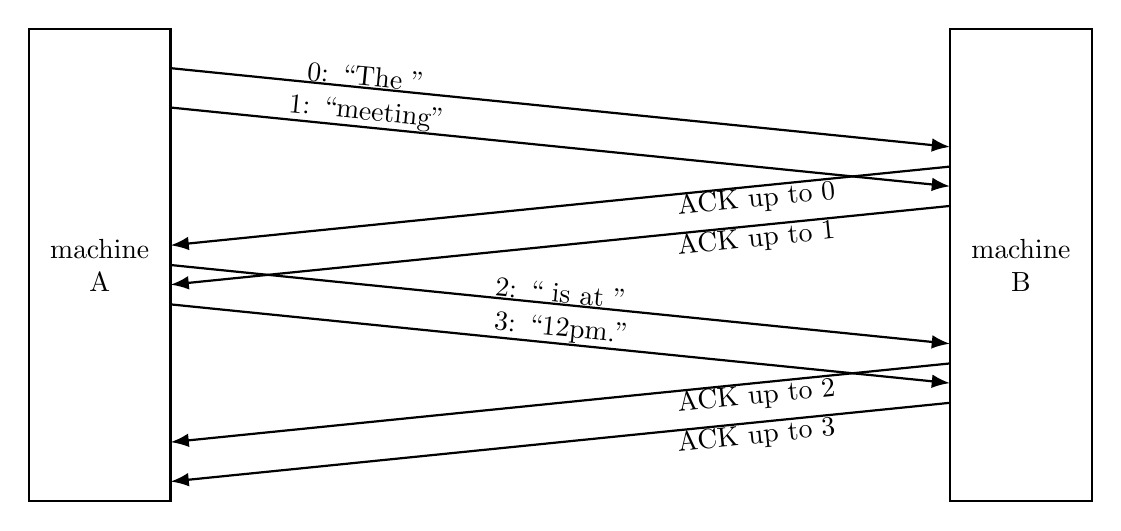
\begin{tikzpicture}
\tikzset{
    box/.style={thick},
    message/.style={draw,thick,-Latex},
    failure/.style={draw,ultra thick,red,cross out,minimum width=1cm,minimum height=1cm},
    every node/.style={inner sep=0.1mm},
}
\begin{scope}[xshift=1cm,x=0.9cm]
\draw[box] (0, 0) rectangle ++(2, -6) 
    node[midway,align=center] {machine\\A};
\draw[box] (13, 0) rectangle ++(2, -6) 
    node[midway,align=center] {machine\\B};
\draw[message] (2, -0.5) -- (13, -1.5) node[pos=0.25,above,sloped] {\myemph{0}: ``The ''};
\draw[message] (13, -1.75) -- (2, -2.75) node[pos=0.25,sloped,below] {ACK up to \myemph{0}};
\draw[message] (2, -1) -- (13, -2) node[pos=0.25, above, sloped] {\myemph{1}: ``meeting''};
\draw[message] (13, -2.25) -- (2, -3.25) node[pos=0.25, sloped,below] {ACK up to \myemph{1}};

% in response to got 0
\draw[message] (2, -3) -- (13, -4) node[pos=0.5, above, sloped] {\myemph{2}: `` is at ''};
\draw[message] (13, -4.25) -- (2, -5.25) node[pos=0.25, sloped,below] {ACK up to \myemph{2}};
% in response to got 1
\draw[message] (2, -3.5) -- (13, -4.5) node[pos=0.5, above, sloped] {\myemph{3}: ``12pm.''};
\draw[message] (13, -4.75) -- (2, -5.75) node[pos=0.25, sloped,below] {ACK up to \myemph{3}};
\end{scope}
\end{tikzpicture}
\begin{itemize}
\item (ACK up to X = ACK X and everything before it)
\item key idea: always have two in flight
\item send next when previous ack'd
\end{itemize}
\end{frame}
